\documentclass[border=0.2cm]{standalone}
\usepackage{tikz}
\begin{document}


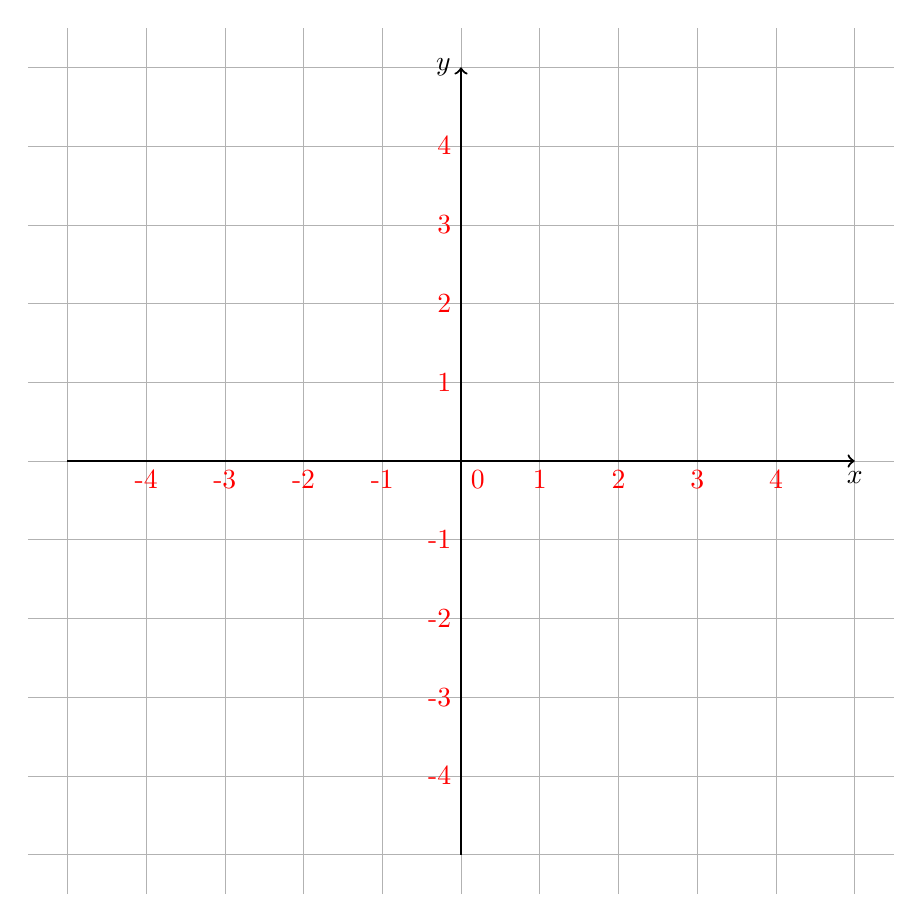
\begin{tikzpicture}
  \draw[help lines,black!30] (-5.5,-5.5) grid (5.5,5.5);
  \draw[thick,->] (0,-5) -- (0,5) node[left]  {$y$};
  \draw[thick,->] (-5,0) -- (5,0) node[below] {$x$};
  \foreach \x in {-4,-3,-2,-1,1,2,3,4} \node[left,color=red] at (0,\x) {\x} node[below,color=red] at (\x,0) {\x};
  \node[below right,color=red] at (0,0) {0}; 
  \end{tikzpicture}



\end{document}